\documentclass[a4paper,12pt]{article}

\usepackage[pdftex]{graphicx}
\usepackage[pdftex,breaklinks=true,colorlinks=true,linkcolor=black,filecolor=blue,urlcolor=blue]{hyperref}
\usepackage{color}
\usepackage[paper=a4paper,hmargin=2cm,vmargin=3cm]{geometry}
\usepackage{lscape}
\usepackage{amsmath}
\usepackage{listings}
\usepackage{fancyhdr}
\usepackage{subfig}
\usepackage{pdflscape}

% Paragraph style
\setlength\parindent{0in}
\setlength\parskip{0.1in}

% URL style
\def\UrlFont{\small\tt}

\lstset{breaklines=true,basicstyle=\small,tabsize=3,numbers=left,numberstyle=\tiny,numbersep=5pt,emptylines=1}

% Setup fancy headings - copied from lshort
\pagestyle{fancy}
% with this we ensure that the chapter and section
% headings are in lowercase.
\renewcommand{\sectionmark}[1]{%
        \markright{\thesection\ #1}}
\fancyhf{} % delete current header and footer
\fancyhead[LE,RO]{\bfseries\thepage}
\fancyhead[LO]{\bfseries\rightmark}
\fancyhead[RE]{\bfseries\leftmark}
\renewcommand{\headrulewidth}{0.5pt}
\renewcommand{\footrulewidth}{0pt}
\addtolength{\headheight}{0.5pt} % space for the rule
\fancypagestyle{plain}{%
   \fancyhead{} % get rid of headers on plain pages
   \renewcommand{\headrulewidth}{0pt} % and the line
}

%opening
\title{COMP6026 Assignment 2 \\
An Evolutionary Approach to Tetris}
\author{David Sansome $<$ds505$>$}

\begin{document}
\bibliographystyle{plain}

\maketitle

\begin{abstract}

This report describes the design, implementation and results of an evolutionary
algorithm that plays the popular game of Tetris \cite{AboutTetris}.
Tetris is a falling-block game where the aim is to survive as long as possible
by dropping blocks (\emph{Tetraminos}) into a fixed-size board.
A row is cleared from the board if it is completely filled, and the game ends
when there is no more room in the board for new blocks.
The challenge therefore is to place blocks in such a way as to minimize holes
in the board and to clear as many rows as possible.

The algorithm used is as described by Mandl et.\ al \cite{Mandl2005}.
At each step of the game the computer evaluates all possible subsequent boards
and chooses the best move based on a rating function.
This function is a weighted sum of various board attributes, such as the height
of filled cells and the number of holes in the board.
The algorithm evolves the weights used in this function and finds sets of
weights that lead to longer games of Tetris.

Our implementation uses fitness proportional selection and uniform crossover.

\end{abstract}

\clearpage
\tableofcontents

\section{Methods}

\subsection{Representation of Individuals}

Each individual in the population is essentially a different \emph{board
rating function}.
The individual uses its board rating function at each step of the game to
decide where to place the next block, choosing the move that will lead to the
board with the best score.
Individuals with better board rating functions will therefore make better moves
and last longer than the other individuals.

The board rating function is a weighted sum of the following six criteria:

\begin{enumerate}
  \item \emph{Pile Height}: The total height of the Tetris board, measured from
      the bottom of the board to the highest occupied cell.
  \item \emph{Holes}: The number of unoccupied cells that have at least one
      occupied cell above them.
  \item \emph{Connected Holes}: Same as \emph{Holes}, except vertically
      connected unoccupied cells only count as one connected hole.
  \item \emph{Removed Lines}: The number of lines that were cleared in the last
      step to get to the current board.
  \item \emph{Altitude Difference}: The difference between the highest occupied
      cell and the lowest free cell that is directly reachable from the top.
  \item \emph{Maximum Well Depth}: The depth of the deepest well on the board.
      A well is a vertical group of unoccupied cells with a width of one,
      reachable from the top and with other filled cells on both sides.
\end{enumerate}

\begin{figure}[hb]
  \centering
  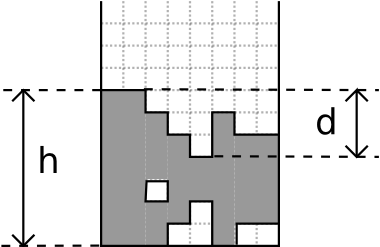
\includegraphics[width=5cm]{boards1.png}
  \caption{A Tetris board showing two of the rating criteria.  $h$ is
      the \emph{Pile Height}, or distance from the bottom of the board to
      the highest occupied cell.  $d$ is the \emph{Altitude Difference}, or
      distance from the highest occupied cell to the lowest occupied cell
      reachable from the top of the board.}
  \label{BoardRating}
\end{figure}

The algorithm described by Mandl et.\ al uses these six criteria as well as
an additional six found in Colin Fahey's ``Standard Tetris Application''
\cite{TetrisAI}, however only these original six were used in our
implementation.

The six criteria ($r_i$) are combined to create the overall linear rating
function $R_l(b)$:

\begin{equation}
  R_l(b) = \sum^6_{i=1} w_ir_i(b)
\end{equation}

Mandl describes two other possible rating functions which give a closer
approximation to the way a human player evaluates the Tetris board.
There is no big difference between pile heights of 2 and 4, but a difference
between heights of 15 and 17 has a much bigger influence on the game.
The exponential rating function $R_e(b)$ is useful because it treats these two
scenarios differently.
The third rating function $R_d(b)$ uses a displacement value and caters for the
idea that the optimum value for a certain criteria might not be zero.

\begin{equation}
\label{ExponentialRating}
  R_e(b) = \sum^6_{i=1} w_ir_i(b)^{e_i}
\end{equation}

\begin{equation}
\label{DisplacementRating}
  R_d(b) = \sum^6_{i=1} w_i \lvert r_i(b) - d_i \rvert ^{e_i}
\end{equation}

Although Mandl evaluates all three rating functions, only the straightforward
linear rating function $R_l(b)$ is used in this implementation.

Each individual therefore consists of one \emph{weights} chromosome
($w_1, \ldots, w_6$) with each of $w_i$ being an integer number.

\subsection{Fitness Evaluation}

The fitness of each individual genotype is measured on the phenotype.
In other words, an instance of the board rating function is created and it is
allowed to play a game of Tetris.
The fitness of the rating function is taken to be the number of blocks it
manages to place before the game ends.

Other possible methods of determining fitness include counting cleared lines
and counting ``points'' for different kinds of actions (for example, scoring
bonus points from clearing more than one line with a single block).

\label{LotsOfGamesEach}
There is a strong random component to the success of an individual in a game of
Tetris (due to the randomness of the upcoming Tetraminos), so each individual
is allowed to play a number of games (usually around 12), and the mean number
of blocks placed each time is taken as its fitness.

\subsection{GA Details}

The Genetic Algorithm (GA) written to evolve the weights uses a generational
approach in which each member of the fixed-size population is replaced at the
start of every new generation.
A pseudo-code implementation is shown in Listing \ref{psuedocode}.

\begin{lstlisting}[firstnumber=1,language=c,morekeywords={until,foreach,in},frame=single,mathescape=true,caption={GA pseudo-code},label={psuedocode},float=[htb]]
foreach individual in population
  individual.InitialiseRandom(-1000, 1000)

for 0 $\leq$ generation $<$ kMaxGenerations
  // Each individual plays kNumberOfGames games of Tetris
  foreach individual in population
    individual.fitness = 0
    for 0 $\leq$ game $<$ kNumberOfGames
      individual.fitness += individual.PlayGame()
    individual.fitness /= kNumberOfGames
  
  // A new population is created
  for 0 $\leq$ i $<$ population.size
    do
      parent1 = population.FitnessProportionateSelection()
      parent2 = population.FitnessProportionateSelection()
    until parent1 $\neq$ parent2
    
    child = UniformCrossover(parent1, parent2)
    child.Mutate()
    
    population2[i] = child
    
  population = population2
\end{lstlisting}

The population is first initialised with individuals that have integer weights
randomly chosen from the range $-1000 \ldots 1000$.

Each member of the population then plays a number of games of Tetris to
determine its fitness.
As explained in Section \ref{LotsOfGamesEach} each individual plays more than
one game, and the fitnesses of each (the number of blocks placed in each game)
are averaged.

After the fitness of each individual is known a new population is created.
Two different parents from the old population are selected using fitness
proportionate selection.
A child is created from the two parents using uniform crossover and its genes
are then mutated slightly.
The child is put into the new population, and this is repeated until the new
population is of the desired size.

\subsubsection{Fitness Proportionate Selection}

In fitness proportionate selection the individual's fitness directly determines
its probability of being selected as a parent for the next generation.

The probability of individual $i$ with a fitness $f_i$ being selected is as
follows:

\begin{equation}
  p_i = \frac{f_i}{\Sigma^N_{j=1} f_j}
\end{equation}

Particular care was taken to ensure that the same individual was not selected
as both parents of the new offspring.
To do this, the first parent is excluded from the ``roulette-wheel'' when it is
generated for selecting the second parent.

\subsubsection{Crossover}

Simple uniform crossover is used to combine the two parents and create a new
individual.
Each weight in the offspring has a 50\% chance of coming from the first parent
and a 50\% chance of coming from the second parent.

There seems to be no advantage in using one or two-point crossover in this
application as the chromosome does not contain any ``blocks'', and genes that
are close to each other are not necessarily related.
However if we had selected one of the more complex rating functions (Equations
\ref{ExponentialRating} and \ref{DisplacementRating}) then weights, exponents
and displacements could be grouped and perhaps provide an advantage for one or
two-point crossover.

\subsubsection{Mutation}

Each one of the individual's weights is mutated by a small amount after it is
created.
This is done by multiplying the weight by a random number drawn from a normal
distribution centred around 1.0 and with standard deviation $\sigma = 0.01$.
These parameters were chosen for the normal distribution as they allow for small
variations to occur in the values of the weights while still making it possible
for genes to be virtually turned off as weights to go to 0.

\begin{figure}[htb]
  \centering
  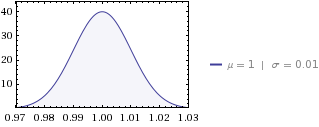
\includegraphics[width=8cm]{normaldist.png}
  \caption{Probability density function of the normal distribution from which
      numbers are taken to mutate an individual's weights. (image from Wolfram
      Alpha \cite{Wolfram})}
  \label{NormalDist}
\end{figure}

Using multiplicative mutation with this normal distribution has the disadvantage
that it becomes impossible for a weight to switch sign (go from positive to
negative or vice versa).
To correct this we should perhaps include an additional probability that the
weight is multiplied by $-1$.

\subsection{Implementation Details}

The implementation was written from scratch in C++.
The Qt toolkit \cite{Qt} was used throughout, and the Boost Random Number
Library \cite{BoostRandom} was used to generate normally distributed random
numbers.
Google perftools \cite{GooglePerftools} was used to identify performance
bottlenecks.

A number of optimisations were made to the code to improve execution speed.
These became necessary with the fitter individuals on larger Tetris boards, as
each game could easily involve hundreds of thousands of blocks.

\begin{enumerate}
  \item The symmetry of various Tetraminos was exploited to reduce the number
      of possible position/orientation combinations to try.
      This reduced the search space by 300\% for the square 2x2 tetramino.
      Figure \ref{Tetraminos} shows the possible orientations for each type
      of Tetramino.
      \begin{figure}[hb]
        \centering
        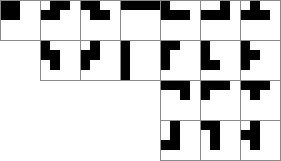
\includegraphics[width=5cm]{tetramino_grid.png}
        \caption{All possible Tetramino configurations}
        \label{Tetraminos}
      \end{figure}
      
  \item The original implementation had a TetrisBoard class that could create
      variable sized boards, with the width and height being specified to the
      constructor at runtime.
      A TetrisBoard has to be created and destroyed for every possible
      position/orientation combination at every step of every game, and so this
      led to almost 25\% of the execution time being spent in malloc and free
      to create these dynamically sized boards.
      A large performance boost was seen by specifying the board size at
      compile time with C++ templates and letting the compiler create the
      boards on the stack.
  
  \item QtConcurrentMap was used to run each game of Tetris in its own thread.
      Because each game can run independently of the others, this leads to
      almost linear performance increases with additional processors.
\end{enumerate}

\section{Results}

The size of a standard tetris board is 10x20, however running experiments on
such a large board is impractical when each generation takes about an hour.
Most tests therefore were run on smaller boards, 6x12 and 8x16 being the most
common.
These smaller boards lead to much harder (and therefore shorter) games of
Tetris.

Unless otherwise stated, the following parameters were used in all experiments:

\begin{center}
  \begin{tabular}{r|l}
    Population size & 128 \\
    Games played per individual & 12 \\
    Total generations & 30 \\
    Board size & 6x12 \\
    Mutation mean ($\mu$) & 1.0 \\
    Mutation standard deviation ($\sigma$) & 0.01 \\
    Initial rating function weights & Random in $-1000 \leq w_i \leq 1000$
  \end{tabular}
\end{center}

\subsection{Varying Standard Deviation}

It was initially suspected that having a large standard deviation value for
the mutation operator was making individuals jump too far away from optima in
the fitness landscape.

The standard deviation was varied between 0.5 and 0.01 to see what effect this
would have on the results.
Figure \ref{StdDev05} shows how the fitness of individuals varied over time
when the highest standard deviation of $\sigma = 0.5$ was used.
It can be seen that the mean fitness varies significantly over time and never
rises above 252.
Figure \ref{StdDev001} shows the lowest standard deviation of $\sigma = 0.01$.
Here we see that the mean fitness rises steadily, eventually reaching its
highest value of 599 after 30 generations.

Higher standard deviation values mean that the weights of each individual
change by a greater amount each time they are mutated.
It seems that if the standard deviation is too high, strong individuals tend to
lose any advantage they once had as they mutate too far away from their original
values that gave them high fitness.

\newcommand{\graphwidth}{11.4cm}
\begin{landscape}
  \begin{figure}[p]
    \centering
    \subfloat[$\sigma = 0.5$]{\label{StdDev05}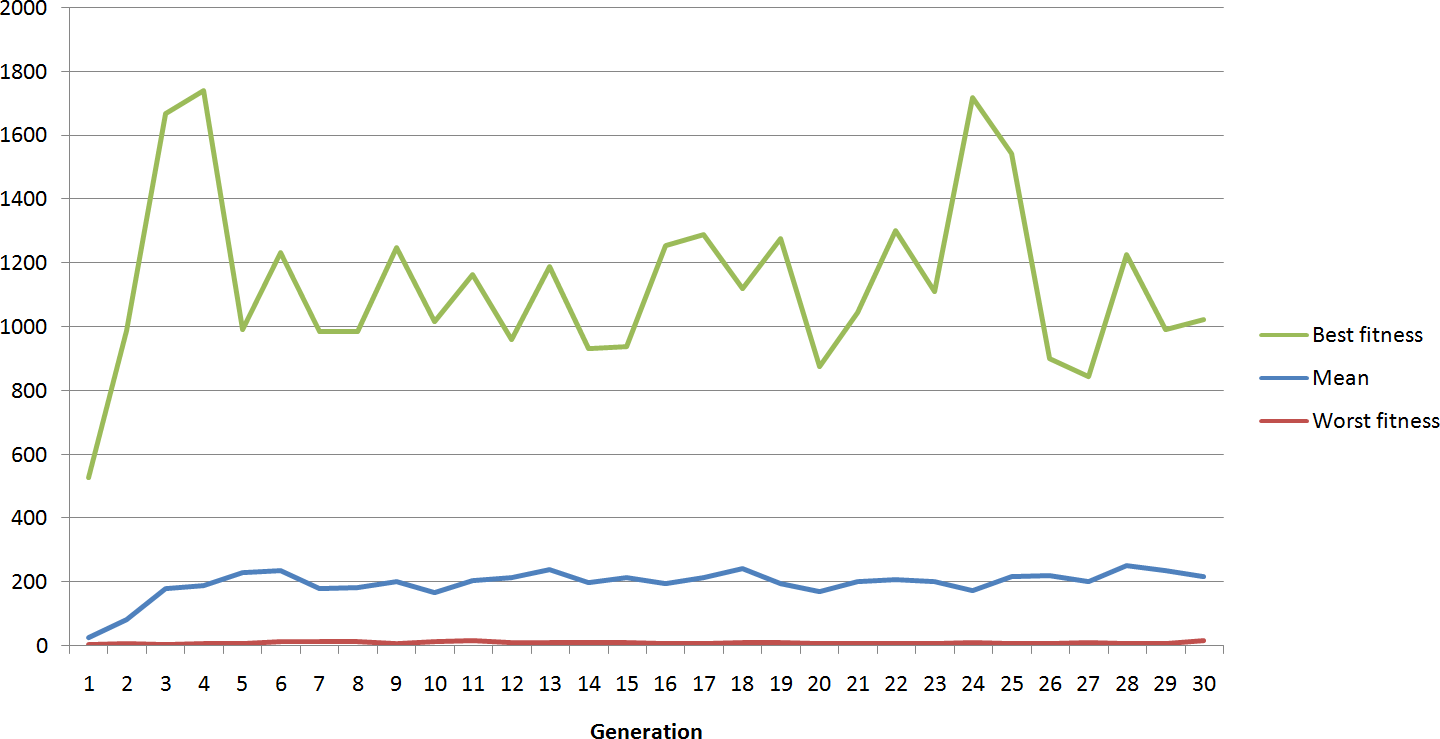
\includegraphics[width=\graphwidth]{results/results4.png}}
    \qquad
    \subfloat[$\sigma = 0.1$]{\label{StdDev01}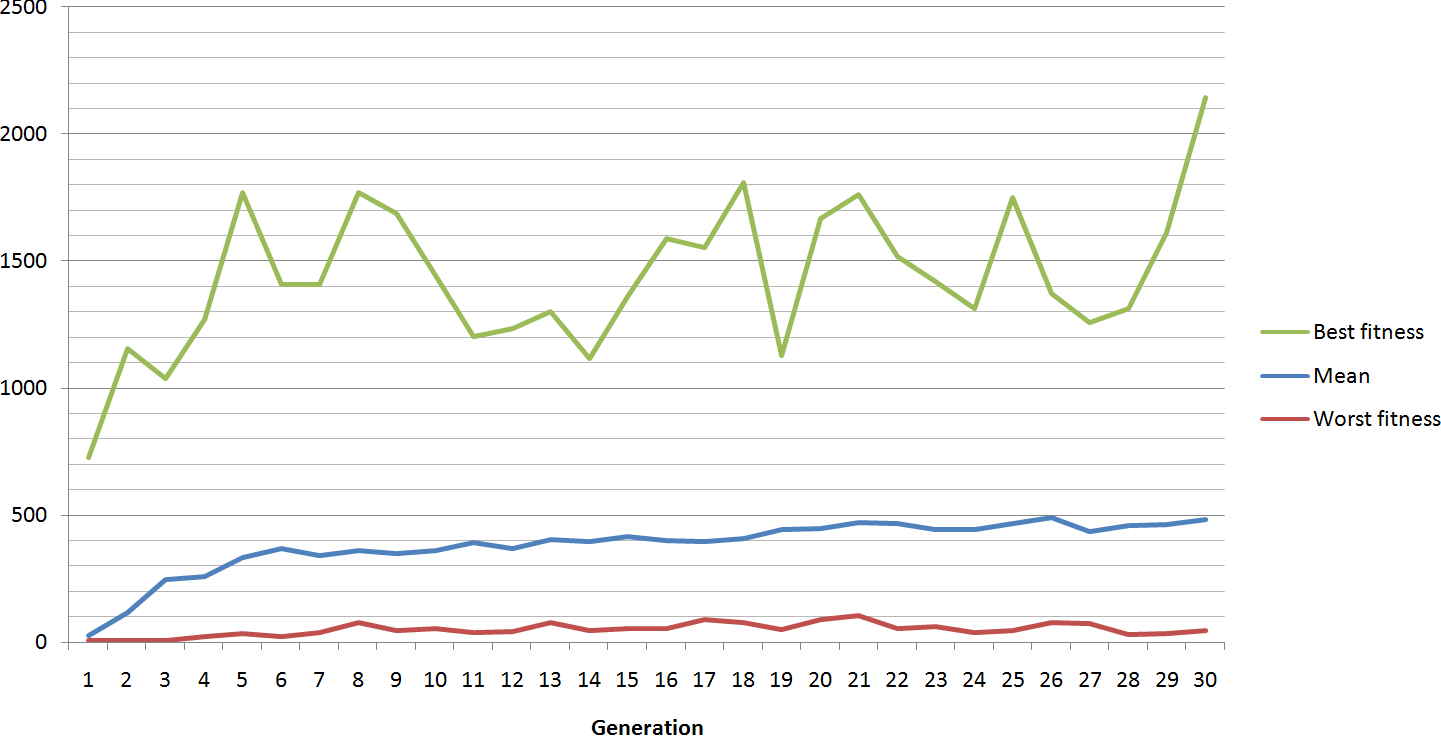
\includegraphics[width=\graphwidth]{results/results1.png}}
    \\
    \subfloat[$\sigma = 0.05$]{\label{StdDev005}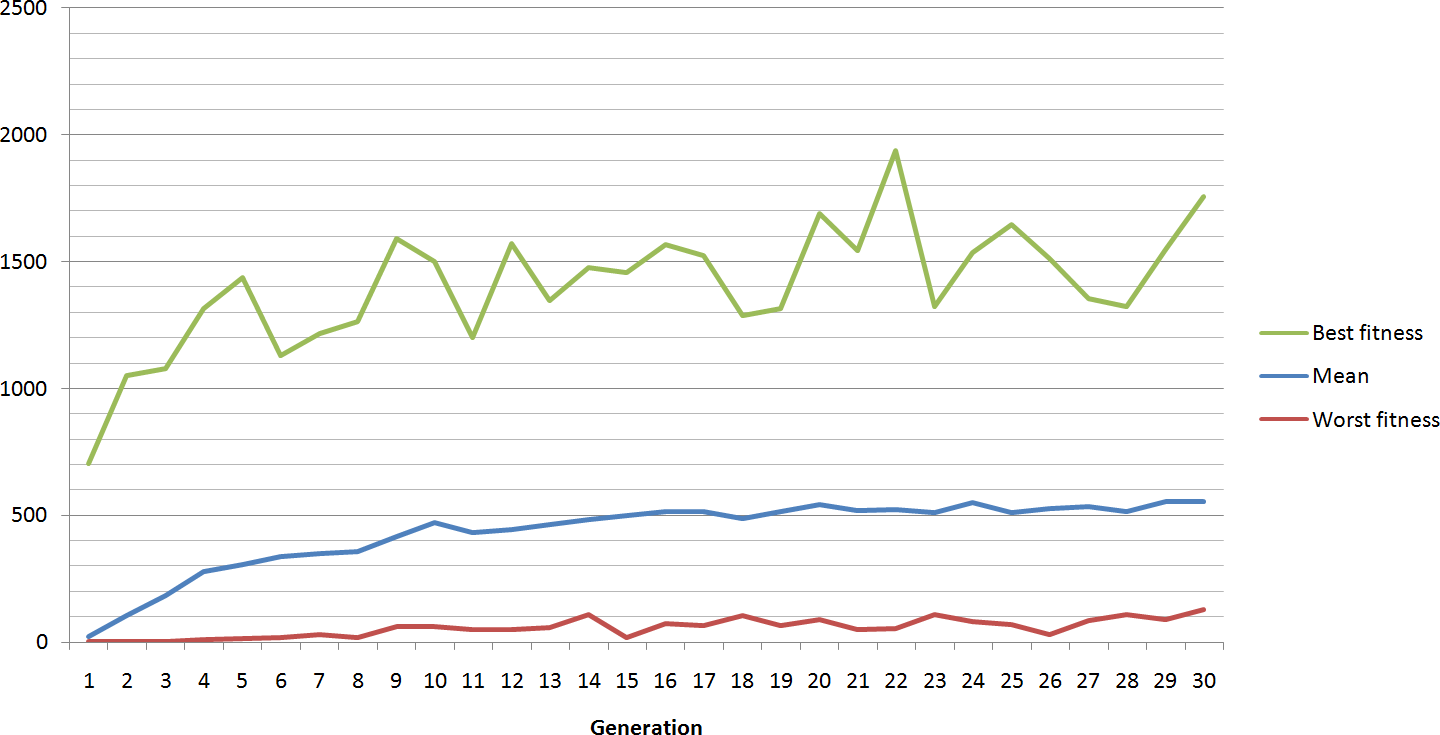
\includegraphics[width=\graphwidth]{results/results2.png}}
    \qquad
    \subfloat[$\sigma = 0.01$]{\label{StdDev001}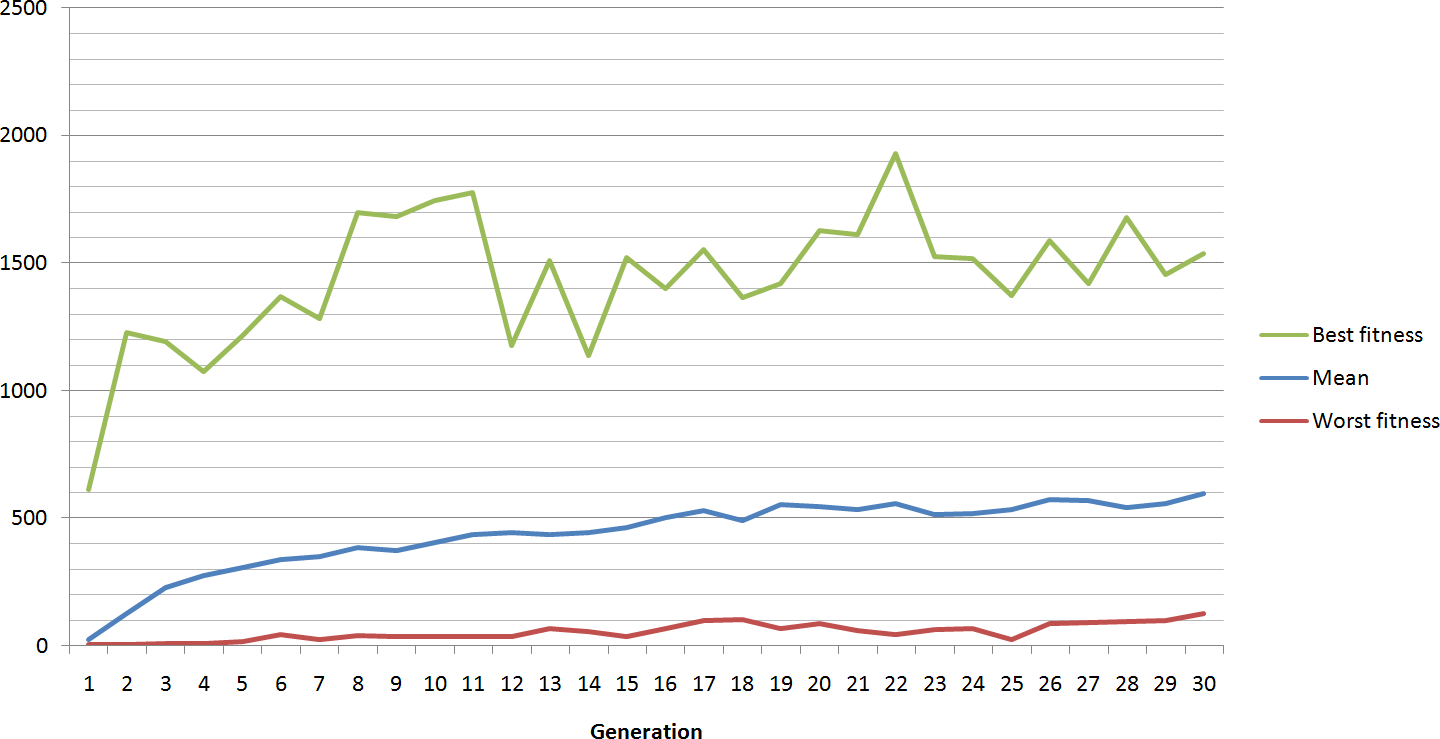
\includegraphics[width=\graphwidth]{results/results3.png}}
    
    \caption{Fitness of individuals over time with varying mutation standard
        deviation.}
    \label{StdDev}
  \end{figure}
\end{landscape}

\subsection{Optimal Weights}

The fittest individual seen on a 6x12 Tetris board managed to place 2145 blocks
before the game was over.
This individual had the following weights:

\begin{center}
  \begin{tabular}{r|l}
    Pile height & 433 \\
    Holes & 739 \\
    Connected holes & 550 \\
    Removed lines & -674 \\
    Altitude difference & 0 \\
    Maximum well depth & 844
  \end{tabular}
\end{center}

The criteria that get the highest weights are the \emph{Maximum well depth} and
\emph{Holes}.
As already observed by human players, it is important to keep wells (the larger
ones can only be cleared by the long 4x1 Tetraminos) and holes (which prevent
you from clearing rows) to a minimum.
Removing lines is obviously advantageous, and the individuals that seek to
remove more lines last longer.

The weighting for altitude difference was reduced to zero, suggesting it has
no bearing whatsoever on gameplay.

\subsection{Larger Boards}

Larger boards tended to give rise to individuals with very similar weights
to the smaller boards.
Two runs from a full-sized 10x20 board are shown below.
These runs took several hours to compute each generation so they were stopped
early, but the mean fitness can be seen to be steadily increasing in much the
same way as the smaller boards.

The fittest individual was able to place 467,739 blocks after 6 generations.

\newcommand{\smallgraphwidth}{8cm}
\begin{figure}[htb]
  \centering
  \subfloat[First run]{\label{Large1}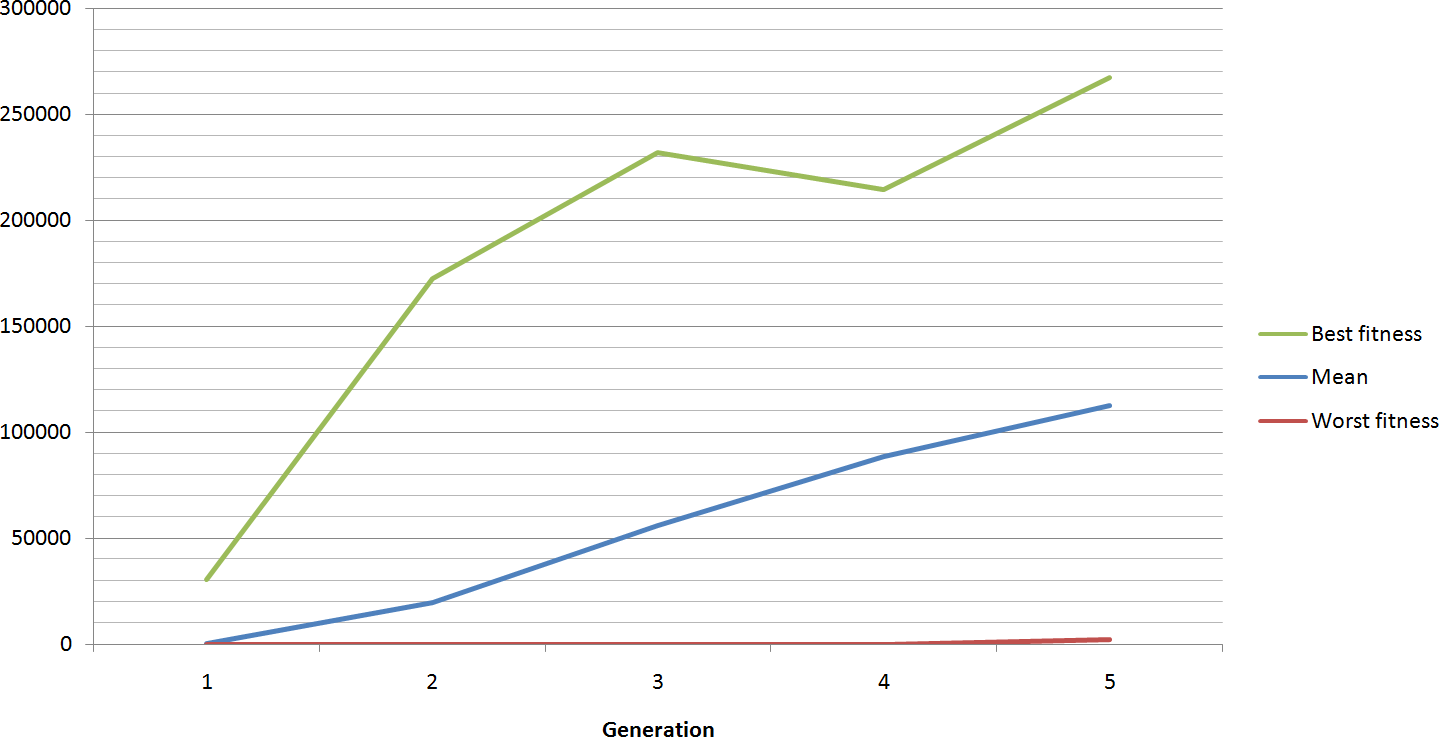
\includegraphics[width=\smallgraphwidth]{results/10x20-results1.png}}
  \qquad
  \subfloat[Second run]{\label{Large2}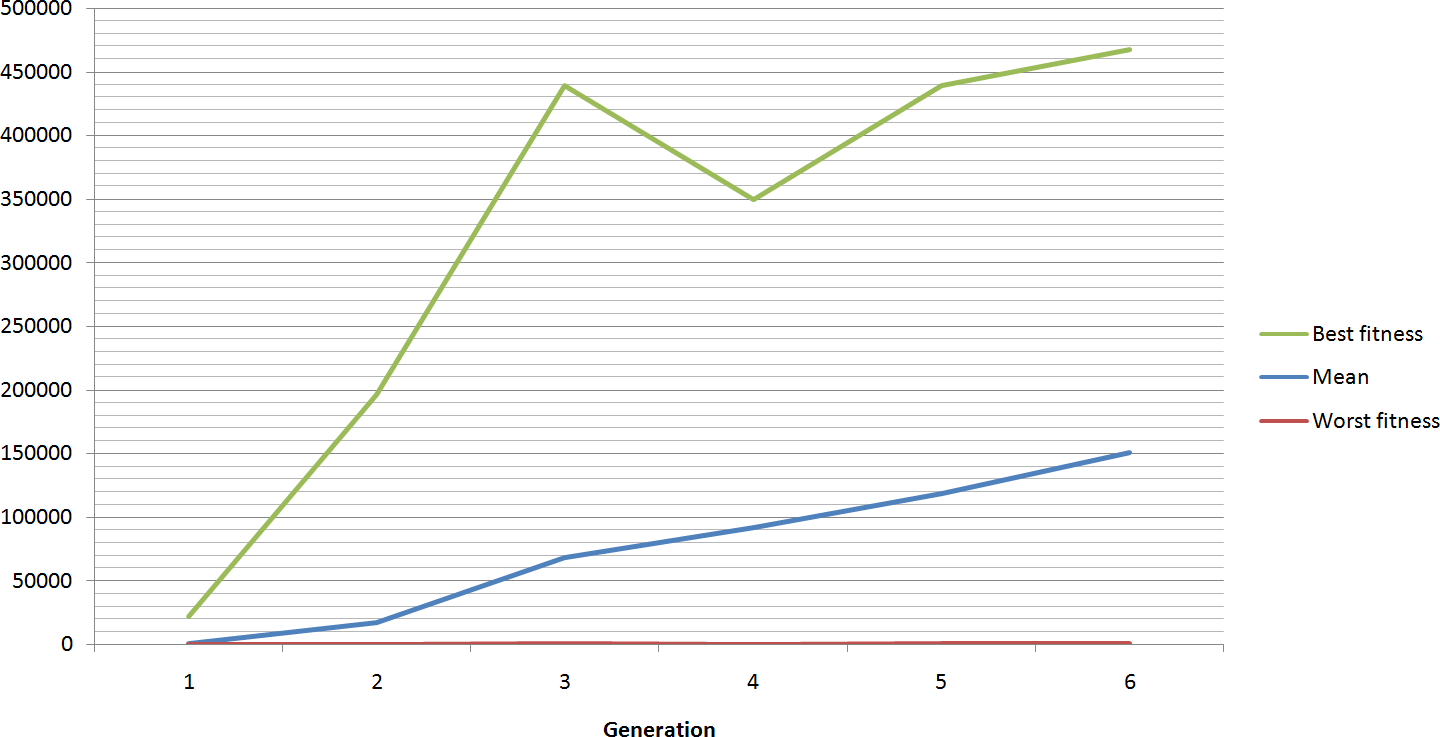
\includegraphics[width=\smallgraphwidth]{results/10x20-results2.png}}

  \caption{Fitness of individuals over time on a full-sized 10x20 Tetris board}
  \label{Large}
\end{figure}

A complete run on a 8x16 board is shown in Figure \ref{Medium}.
The mean fitness seems to rise in a similar way but reaches its maximum sooner
than the smaller board (Figure \ref{StdDev001}).
After generation 12 this population stops any dramatic increases in fitness,
but the smaller board keeps increasing (albeit very slowly) right until the end.

This could be because smaller games of Tetris are much harder so there's more
to gain from small improvements to the weights.

\begin{figure}[h]
  \centering
  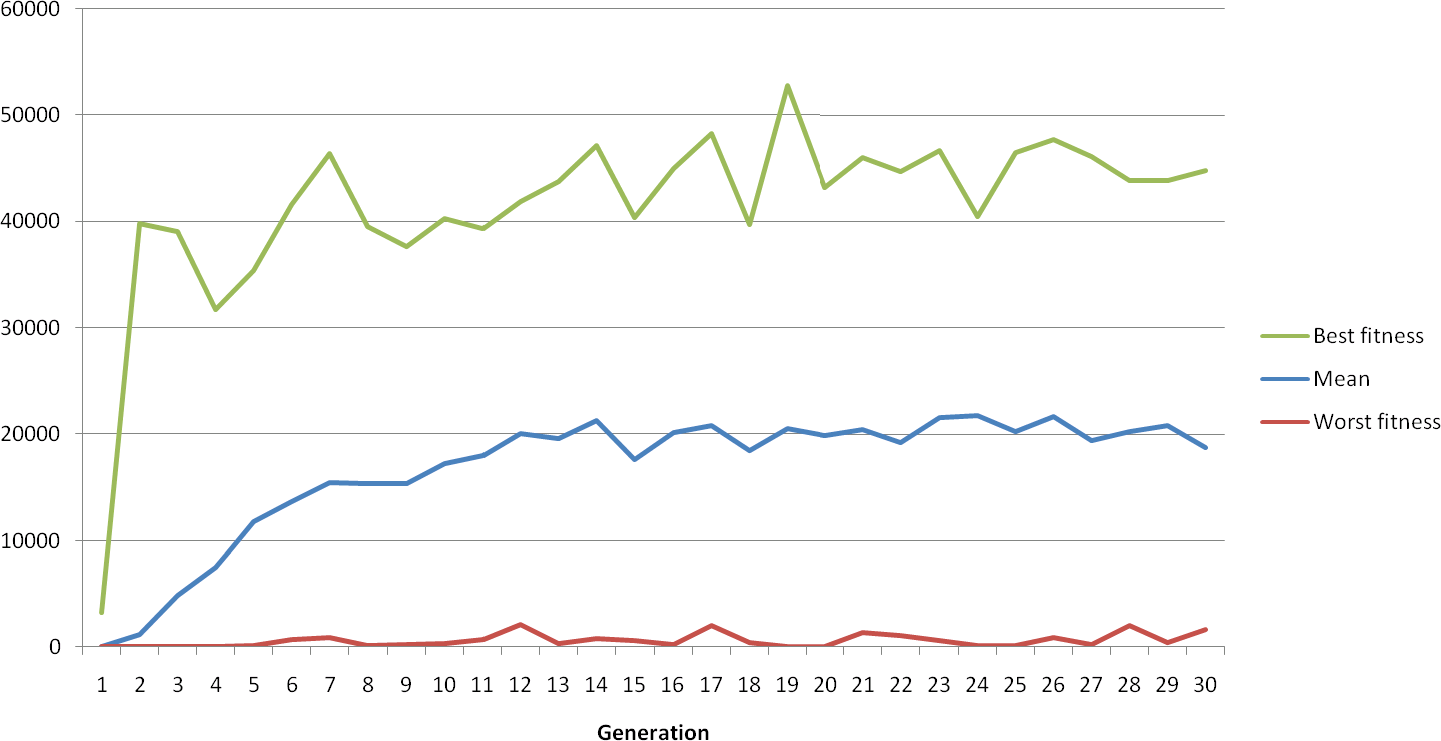
\includegraphics[width=\graphwidth]{results/8x16.png}
  \caption{Fitness of individuals over time on a 8x16 Tetris board}
  \label{Medium}
\end{figure}

The fittest individual in the 8x16 game was seen after 19 generations, and
was able to place 52,814 blocks.

\section{Further Work}

It would be interesting to investigate the effects of co-evolving the
Tetris-playing population against a second population that is trying to create
new types of Tetramino that are more difficult to place successfully.

Each individual in the second population would represent a set of Tetraminos,
and they would all be initialised to the standard set shown in Figure
\ref{Tetraminos}.
The mutation operator for the second population would alter individual
Tetraminos by adding or removing cells to the shape, up to a certain size limit,
and ensuring that each shape remained connected.
Individuals from the Tetris-playing population would then play games against
individuals from the Tetramino-creating population.

The mutation and combination operators for the second population would have the
scope to become much more complicated than those of the Tetris-playing
population.
For example, one-point crossover could be used to merge different halves of
separate Tetraminos together.

The questions to be answered would be:

\begin{enumerate}
  \item Does co-evolution improve the Tetris-players' ability to cope with new
      and unknown shapes?
  \item Will individuals that have undergone co-evolution then also have
      improved their ability to play with the original set of Tetraminos.
\end{enumerate}

In answering these questions, it would also be useful to make the Tetris players
more sophisticated:

\begin{enumerate}
  \item The board rating function should include the additional six criteria
      detailed in Mandl's paper.
  \item The exponential rating function (Equation \ref{ExponentialRating})
      described in Mandl's paper should be used, and the set of exponents
      $e_1, \ldots, e_N$ added to the individuals as an additional genotype to
      be evolved.
      Mandl saw no significant improvements from adding evolvable displacements
      to the exponential rating function (Equation \ref{DisplacementRating}),
      so in our extension we will just use the version of this function without
      displacements.
\end{enumerate}

We will likely see different sets of weights emerging for the more complicated
shapes, as different strategies will be required to play games with them
successfully.
However it seems equally possible that since the board rating criteria are
quite generic (number of holes, pile height, etc.), an individual that is good
at playing with one set of Tetraminos will be just as good as playing with
another set.

\bibliography{../COMP6026}

\appendix
\clearpage
\lstset{language=c++}
\section{Code Listings}

\subsection{main.cpp}
\lstinputlisting{"main.cpp"}

\clearpage
\subsection{engine.h}
\lstinputlisting{"engine.h"}

\subsection{engine.cpp}
\lstinputlisting{"engine.cpp"}

\clearpage
\subsection{game.h}
\lstinputlisting{"game.h"}

\clearpage
\subsection{individual.h}
\lstinputlisting{"individual.h"}

\subsection{individual.cpp}
\lstinputlisting{"individual.cpp"}

\clearpage
\subsection{population.h}
\lstinputlisting{"population.h"}

\subsection{population.cpp}
\lstinputlisting{"population.cpp"}

\clearpage
\subsection{tetrisboard.h}
\lstinputlisting{"tetrisboard.h"}

\clearpage
\subsection{tetramino.h}
\lstinputlisting{"tetramino.h"}

\subsection{tetramino.cpp}
\lstinputlisting{"tetramino.cpp"}

\clearpage
\subsection{testboard.h}
\lstinputlisting{"test_board.h"}

\subsection{testboard.cpp}
\lstinputlisting{"test_board.cpp"}

\end{document}
